\documentclass[10 pt]{article}
\usepackage{tikz}
\usetikzlibrary{arrows}
\usepackage[margin=0.5 in]{geometry}
\usepackage[utf8]{inputenc}
\usepackage{tabu}
\usepackage{color}
\usepackage{xcolor}
\usepackage{listings}
\usepackage{enumitem}
\usepackage{siunitx}
\usepackage{multicol}
\usepackage{titlesec} 

\setlength{\columnsep}{1cm} 
\titleformat{\subsection}[runin]
{\normalfont\large\bfseries}{\thesubsection}{1em}{}
\titleformat{\subsubsection}[runin]
{\normalfont\normalsize\bfseries}{\thesubsubsection}{1em}{}

\title{\textbf {Estructuras de Datos 1 - ST0245\\Examen Parcial 2 - Martes (032)
}}
\author{Nombre ..............................\\
		Departamento de Informática y Sistemas\\
		Universidad EAFIT\\}
\date{Octubre 22 de 2019}
\begin{document}
\lstdefinestyle{customc}{
	language=Java, 
	numbers=left, 
	showspaces=false,
    showstringspaces=false, 
    tabsize=2, 
    breaklines=true,
    xleftmargin=5.0ex,
}
\lstset{escapechar=@,style=customc, numbers=left, stepnumber = 1} 
\maketitle

\textbf{En las preguntas de selección múltiple, una respuesta incorrecta tendrá
una deducción de 0.2 puntos en la nota final. Si dejas la pregunta sin
responder, la nota será de 0.0. Si no conoces la respuesta, no adivines.}


\begin{multicols}{2}


\section{1. Tablas de Hash 20\%}
En los videojuegos, las tablas de hash se usan para guardar la información de las armas; por ejemplo,
su ataque, su velocidad y su duración. Considera la siguiente función de hash para cadenas de caracteres.
La constante \texttt{TABLE\_SIZE} representa el tamaño máximo del arreglo con el que se representamente
internamente la tabla de hash.

{\footnotesize
\begin{lstlisting}
private int funcionHash(String k){
  return ((int) k.charAt(0)) % TABLE_SIZE;
}
\end{lstlisting}
}
\begin{enumerate}[label=\alph*]
	\item (10\%) ¿Qué problema presenta esta función hash? Las cadenas...
	{\small
	\begin{enumerate}[label=\roman*]
		% Respuesta: Todas las cadenas que inician con la misma letra colisionan
		\item  que terminan con la misma letra colisionan
		\item  que inician con la misma letra colisionan
		\item  cuya suma de los caracteres es la misma colisionan
		\item  que tienen los mismos caracteres colisionan
	\end{enumerate}
	}
	\item (10\%) ¿Cuál es la complejidad asintótica, en el peor de los casos, de \texttt{funcionHash(k)}? Donde $n$ es la longitud de la cadena $k$.
	\begin{enumerate}[label=\roman*]
		% Respuesta: $O(1)$
		\item $O(n)$
		\item $O(n^2)$
		\item $O(n\log n)$
		\item $O(1)$
	\end{enumerate}
\end{enumerate}



\section{2. Listas 20\%}
Liko escribió un nuevo método para una lista simplemente enlazada. Desafortunamente, Liko olvidó
qué hace el método. ¿Podrías ayudarnos a decifrar qué retorna el método \texttt{mistery} y su complejidad?
{\footnotesize
\begin{lstlisting}
class Node { 
   int data; 
   Node next; 
   Node(int d) { data = d; } 
} 
class AlgoritmosDeListas { 
 public static Node mistery(Node node) { 
   Node prev = null; 
   Node current = node; 
   Node next = null; 
   while (current != null) { 
     next = current.next; 
     current.next = prev; 
     prev = current; 
     current = next; 
   } 
   node = prev; 
   return node; 
 }
}
\end{lstlisting}
}
\begin{enumerate}[label=\alph*]
	\item (10\%) ¿Qué retorna el algoritmo anterior?
	\begin{enumerate}[label=\roman*]
		% Respuesta: la lista con los elementos en orden inverso
		\item La lista ordenada de mayor a menor
		\item La lista con los elementos en orden inverso
		\item La lista ordenada de menor a mayor
		\item La misma lista 
	\end{enumerate}
	\item (10\%) ¿Cuál es la complejidad asintótica, en el peor de los casos, del algoritmo anterior? Donde $n$ es la longitud de la lista que inicia con el nodo \texttt{node}.
	\begin{enumerate}[label=\roman*]
		% Respuesta: $O(n)$
		\item $O(n)$
		\item $O(n^2)$
		\item $O(n\log n)$
		\item $O(n \times (\log n)^2)$
	\end{enumerate}
\end{enumerate}



\section{3. Grafos  20\%}
Considera el siguiente grafo no dirigido:
\begin{center}
		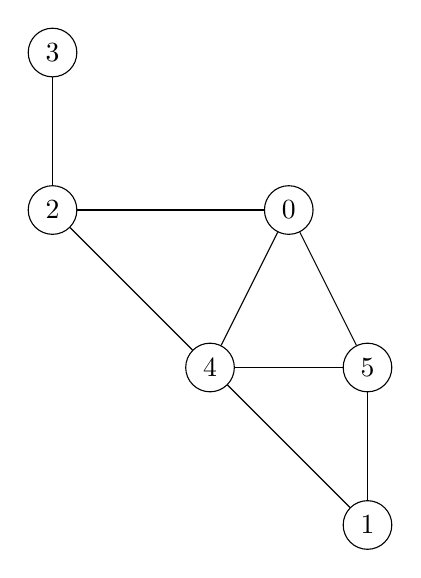
\begin{tikzpicture}
		
		\tikzset{vertex/.style = {shape=circle,draw,minimum size=1.5em}}
		\tikzset{edge/.style = {-,> = latex'}}
		\node[vertex] (0) at (0,0)  {0};
		\node[vertex] (5) at (1,-2)  {5};
		\node[vertex] (4) at (-1,-2)  {4};
		\node[vertex] (1) at (1,-4)  {1};
		\node[vertex] (2) at (-3, 0) {2};
		\node[vertex] (3) at (-3, 2) {3};
		%edges
		\draw[edge] (0) to (4);	
		\draw[edge] (0) to (5);
		\draw[edge] (5) to (4);
		\draw[edge] (5) to (1);
		\draw[edge] (4) to (1);
		\draw[edge] (4) to (2);
		\draw[edge] (0) to (2);
		\draw[edge] (2) to (3);
		\end{tikzpicture}
	\end{center}
	\begin{enumerate}[label=\alph*)]
		\item (10\%) ¿Cuál es un recorrido de \emph{búsqueda primero en profundidad} del grafo anterior, si como nodo inicial se toma el nodo 1?
		\begin{enumerate}[label=\roman*)]
			\item 1, 5, 0, 3, 2, 4
			\item 1, 4, 5, 0, 2, 3
			\item 1, 4, 0, 3, 5, 2
			\item 1, 5, 4, 0, 3, 2
		\end{enumerate}
	    \item (10\%) ¿Cuál es un recorrido de \emph{búsqueda primero en amplitud} del grafo anterior, si se toma como nodo inicial el nodo 1?
	    \begin{enumerate}[label=\roman*)]
	    	\item 1, 4, 5, 0, 2, 3
	    	\item 1, 5, 0, 2, 3, 4
	    	\item 1, 4, 2, 0, 3, 5
	    	\item 1, 3, 0, 4, 5, 2
	    \end{enumerate}
	\end{enumerate}

\section{4. Pilas 20\%}
Kefo escribió un nuevo método para evaluar una expresión aritmética en 
\emph{notación polaca inversa}, pero se le borraron algunas líneas y no había hecho \emph{commit} en git. La notación polaca inversa evita el uso de
paréntesis; para lograrlo primero se colocan los operandos y luego 
los operadores. Considera los siguientes ejemplos:
\begin{itemize}
  \item Esta entrada [``2'', ``1'', ``+'', ``3'', ``*''], es equivalente a esta expresión $((2 + 1) * 3)$  y la respuesta es $9$
  \item Esta entrada [``4'', ``13'', ``5'', ``/'', ``+''], es equivalente a  $(4 + (13 / 5))$ y la respuesta es $6$
\end{itemize}

{\footnotesize
\begin{lstlisting}
int evalRPN(String[] expression) {
  int returnValue = 0;
  String operators = "+-*/";
  Stack<String> stack = new Stack<String>();
  for(String t : expression){
    if(!operators.contains(t)){
        .............;
    }else{
      int a = Integer.valueOf(stack.pop());
      int b = Integer.valueOf(stack.pop());
      int index = operators.indexOf(t);
      switch(index){
       case 0:
        stack.push(String.valueOf(a+b));
        break;
       case 1:
        stack.push(String.valueOf(b-a));
        break;
       case 2:
        stack.push(String.valueOf(a*b));
        break;
       case 3:
        stack.push(String.valueOf(b/a));
        break;
       }
    }
  }
  returnValue = Integer.valueOf(............);
  return returnValue; 
}
\end{lstlisting}
}

\begin{enumerate}[label=\alph*]
	\item (10\%) Completa, por favor, la línea 7\\
	% Respuesta:  stack.push(t);
	$\rule{8cm}{0.15mm}$

	\item (10\%) Completa, por favor, la línea 28\\
	% Respuesta:  stack.pop()
	$\rule{8cm}{0.15mm}$
\end{enumerate}

El método \texttt{String.valueOf(a)} convierte el entero $a$ en un String.
El ciclo \texttt{for(String t : expression)} se lee como ``para cada \texttt{String t} en el arreglo \texttt{expression}, de izquierda a derecha, haga...'' El método \texttt{A.contains(b)} retorna verdadero si $b$ está en A; de lo contrario, falso. El método  \texttt{operators.indexOf(t)} retorna la posición en la cadena \texttt{operators} donde aparece el elemento $t$.

% int evalRPN(String[] tokens) {
%   int returnValue = 0;
%   String operators = "+-*/";
%   Stack<String> stack = new Stack<String>();
%   for(String t : tokens){
%     if(!operators.contains(t)){
%         stack.push(t);
%     }else{
%                 int a = Integer.valueOf(stack.pop());
%                 int b = Integer.valueOf(stack.pop());
%                 int index = operators.indexOf(t);
%                 switch(index){
%                     case 0:
%                         stack.push(String.valueOf(a+b));
%                         break;
%                     case 1:
%                         stack.push(String.valueOf(b-a));
%                         break;
%                     case 2:
%                         stack.push(String.valueOf(a*b));
%                         break;
%                     case 3:
%                         stack.push(String.valueOf(b/a));
%                         break;
%                 }
%             }
%         }
%         returnValue = Integer.valueOf(stack.pop());
%         return returnValue; 
% }


\section{5. Árboles binarios de búsqueda 20\%}
Considera el siguiente árbol:
\begin{center}
	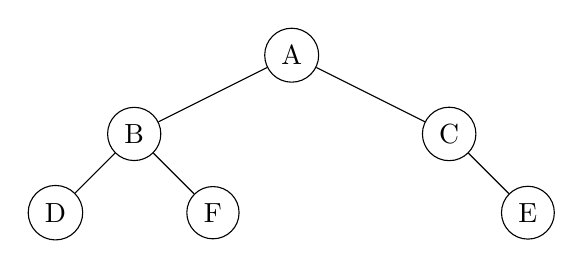
\begin{tikzpicture}
	\tikzset{vertex/.style = {shape=circle,draw,minimum size=1.5em}}
	\tikzset{edge/.style = {-,> = latex'}}
	\node[vertex] (0) at (0,0)  {A};
	\node[vertex] (1) at (-2,-1)  {B};
	\node[vertex] (2) at (2, -1) {C};
	\node[vertex] (3) at (-3, -2) {D};
	\node[vertex] (4) at (3, -2) {E};
	\node[vertex] (5) at (-1, -2) {F};
	%edges
	\draw[edge] (0) to (1);
	\draw[edge] (0) to (2);
	\draw[edge] (1) to (3);
	\draw[edge] (1) to (5);
	\draw[edge] (2) to (4);
	\end{tikzpicture}
\end{center}
\begin{enumerate}[label=\alph*]
	\item (10\%) ¿Qué configuración de vértices $[A, B, C, D, E, F]$ hacen el árbol anterior sea un \emph{árbol binario de búsqueda}?
	\begin{enumerate}[label=\roman*]
		% Respuesta: iv) $[8, 6, 9, 4, 7, 10]$
		\item $[5, 7, 1, 4, 9, 8]$
		\item $[-1, 4, 9, 8, 6, 5]$
		\item $[11, 4, 7, 9, 3, 1]$
		\item $[8, 6, 9, 4, 7, 10]$
	\end{enumerate}
	\item (10\%) ¿Cuál es la complejidad asintótica, en el peor de los casos, de encontrar un elemento en un árbol de búsqueda binaria que NO se autobalancea?
	\begin{enumerate}[label=\roman*]
		% Respuesta: i) $O(n)$
		\item $O(n)$
		\item $O(1)$
		\item $O(\log n)$
		\item $O(n \log n)$
	\end{enumerate}
	
\end{enumerate}
\end{multicols}
\end{document}